\documentclass[a4paper,ngerman,landscape,30pt]{scrartcl}

\usepackage[utf8]{inputenc}
\usepackage{amsmath}

\usepackage[ngerman]{babel}
\usepackage{hyperref}

\usepackage{graphicx}

\usepackage[protrusion=true,expansion=true]{microtype}
\usepackage{lmodern}

\setlength\parskip{\medskipamount}
\setlength\parindent{0pt}

\usepackage{geometry}
\geometry{tmargin=1.5cm,bmargin=1.0cm,lmargin=2.5cm,rmargin=2.5cm}

\pagestyle{empty}

\begin{document}

\newcommand{\page}[1]{
  \begin{center}
    \Huge\sffamily
    #1%
    \vfill
    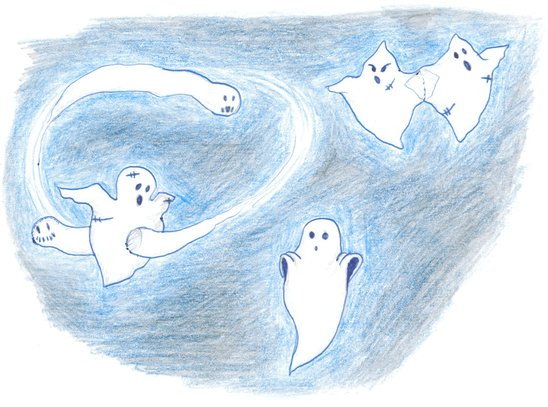
\includegraphics[scale=2]{images/phantome}
  \end{center}
  \newpage
}

\page{Jedes Konzept ist eine \textbf{Kan-Erweiterung}.}

\page{\textbf{Adjunktionen} \\ sind überall.}

\page{Manche Dinge kann man nicht derivieren.}
\page{Für alles andere gibt es Homotopische Algebra.}

\page{Wenn abgeleitete Kategorien nicht ausreichen:}
\page{\textbf{Modellkategorien.}}

\page{Leitest du noch Funktionen ab \ldots}
\page{oder schon \textbf{Funktoren}?}

\page{
  Eine \textbf{gute Kategorie} topologischer Räume:
  die kompakt erzeugten.
}

\page{
  \textbf{Modellkategorien:} \\
  \huge
  der richtige Rahmen zur Lokalisierung von Kategorien.
}

\page{
  \textbf{Vollständige metrische Räume?} \\
  \large
  Ah, du meinst metrische Räume lokalisiert an den Bilipschitzabbildungen mit
  dichtem Bild!
  Willkommen in der fabelhaften Welt der \textbf{Kategorienlokalisierung}.
}

\page{
  \textbf{Garben?} \\
  \Large
  Ah, du meinst Prägarben lokalisiert an den halmweisen Isomorphismen! \\
  Willkommen in der wunderbaren Welt der \textbf{Kategorienlokalisierung}.
}

\page{
  Weil man \textbf{Einhängung} invertierbar machen möchte:
  \textbf{Spektren}.
}

\page{Was ist besser als Modellkategorien?}
\page{\textbf{Monoidale Modellkategorien!}}

\begin{center}
  \Huge\sffamily
  Modellkategorien
  \vfill
  
\includegraphics[scale=1]{images/derive-all-the-functors}
\end{center}
\newpage

\begin{center}
  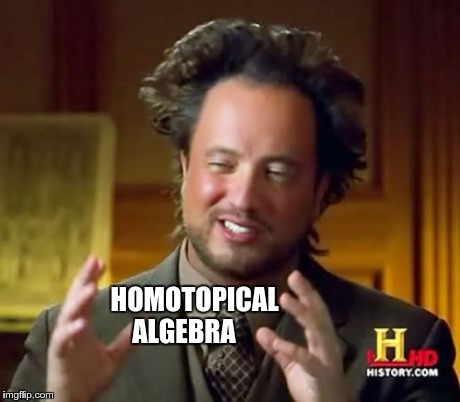
\includegraphics[scale=1.3]{images/aliens}
\end{center}

\end{document}
